% Options for packages loaded elsewhere
\PassOptionsToPackage{unicode}{hyperref}
\PassOptionsToPackage{hyphens}{url}
\PassOptionsToPackage{dvipsnames,svgnames,x11names}{xcolor}
%
\documentclass[
  letterpaper,
  DIV=11,
  numbers=noendperiod]{scrartcl}

\usepackage{amsmath,amssymb}
\usepackage{iftex}
\ifPDFTeX
  \usepackage[T1]{fontenc}
  \usepackage[utf8]{inputenc}
  \usepackage{textcomp} % provide euro and other symbols
\else % if luatex or xetex
  \usepackage{unicode-math}
  \defaultfontfeatures{Scale=MatchLowercase}
  \defaultfontfeatures[\rmfamily]{Ligatures=TeX,Scale=1}
\fi
\usepackage{lmodern}
\ifPDFTeX\else  
    % xetex/luatex font selection
\fi
% Use upquote if available, for straight quotes in verbatim environments
\IfFileExists{upquote.sty}{\usepackage{upquote}}{}
\IfFileExists{microtype.sty}{% use microtype if available
  \usepackage[]{microtype}
  \UseMicrotypeSet[protrusion]{basicmath} % disable protrusion for tt fonts
}{}
\makeatletter
\@ifundefined{KOMAClassName}{% if non-KOMA class
  \IfFileExists{parskip.sty}{%
    \usepackage{parskip}
  }{% else
    \setlength{\parindent}{0pt}
    \setlength{\parskip}{6pt plus 2pt minus 1pt}}
}{% if KOMA class
  \KOMAoptions{parskip=half}}
\makeatother
\usepackage{xcolor}
\setlength{\emergencystretch}{3em} % prevent overfull lines
\setcounter{secnumdepth}{-\maxdimen} % remove section numbering
% Make \paragraph and \subparagraph free-standing
\makeatletter
\ifx\paragraph\undefined\else
  \let\oldparagraph\paragraph
  \renewcommand{\paragraph}{
    \@ifstar
      \xxxParagraphStar
      \xxxParagraphNoStar
  }
  \newcommand{\xxxParagraphStar}[1]{\oldparagraph*{#1}\mbox{}}
  \newcommand{\xxxParagraphNoStar}[1]{\oldparagraph{#1}\mbox{}}
\fi
\ifx\subparagraph\undefined\else
  \let\oldsubparagraph\subparagraph
  \renewcommand{\subparagraph}{
    \@ifstar
      \xxxSubParagraphStar
      \xxxSubParagraphNoStar
  }
  \newcommand{\xxxSubParagraphStar}[1]{\oldsubparagraph*{#1}\mbox{}}
  \newcommand{\xxxSubParagraphNoStar}[1]{\oldsubparagraph{#1}\mbox{}}
\fi
\makeatother


\providecommand{\tightlist}{%
  \setlength{\itemsep}{0pt}\setlength{\parskip}{0pt}}\usepackage{longtable,booktabs,array}
\usepackage{calc} % for calculating minipage widths
% Correct order of tables after \paragraph or \subparagraph
\usepackage{etoolbox}
\makeatletter
\patchcmd\longtable{\par}{\if@noskipsec\mbox{}\fi\par}{}{}
\makeatother
% Allow footnotes in longtable head/foot
\IfFileExists{footnotehyper.sty}{\usepackage{footnotehyper}}{\usepackage{footnote}}
\makesavenoteenv{longtable}
\usepackage{graphicx}
\makeatletter
\def\maxwidth{\ifdim\Gin@nat@width>\linewidth\linewidth\else\Gin@nat@width\fi}
\def\maxheight{\ifdim\Gin@nat@height>\textheight\textheight\else\Gin@nat@height\fi}
\makeatother
% Scale images if necessary, so that they will not overflow the page
% margins by default, and it is still possible to overwrite the defaults
% using explicit options in \includegraphics[width, height, ...]{}
\setkeys{Gin}{width=\maxwidth,height=\maxheight,keepaspectratio}
% Set default figure placement to htbp
\makeatletter
\def\fps@figure{htbp}
\makeatother
% definitions for citeproc citations
\NewDocumentCommand\citeproctext{}{}
\NewDocumentCommand\citeproc{mm}{%
  \begingroup\def\citeproctext{#2}\cite{#1}\endgroup}
\makeatletter
 % allow citations to break across lines
 \let\@cite@ofmt\@firstofone
 % avoid brackets around text for \cite:
 \def\@biblabel#1{}
 \def\@cite#1#2{{#1\if@tempswa , #2\fi}}
\makeatother
\newlength{\cslhangindent}
\setlength{\cslhangindent}{1.5em}
\newlength{\csllabelwidth}
\setlength{\csllabelwidth}{3em}
\newenvironment{CSLReferences}[2] % #1 hanging-indent, #2 entry-spacing
 {\begin{list}{}{%
  \setlength{\itemindent}{0pt}
  \setlength{\leftmargin}{0pt}
  \setlength{\parsep}{0pt}
  % turn on hanging indent if param 1 is 1
  \ifodd #1
   \setlength{\leftmargin}{\cslhangindent}
   \setlength{\itemindent}{-1\cslhangindent}
  \fi
  % set entry spacing
  \setlength{\itemsep}{#2\baselineskip}}}
 {\end{list}}
\usepackage{calc}
\newcommand{\CSLBlock}[1]{\hfill\break\parbox[t]{\linewidth}{\strut\ignorespaces#1\strut}}
\newcommand{\CSLLeftMargin}[1]{\parbox[t]{\csllabelwidth}{\strut#1\strut}}
\newcommand{\CSLRightInline}[1]{\parbox[t]{\linewidth - \csllabelwidth}{\strut#1\strut}}
\newcommand{\CSLIndent}[1]{\hspace{\cslhangindent}#1}

\KOMAoption{captions}{tableheading}
\makeatletter
\@ifpackageloaded{caption}{}{\usepackage{caption}}
\AtBeginDocument{%
\ifdefined\contentsname
  \renewcommand*\contentsname{Table of contents}
\else
  \newcommand\contentsname{Table of contents}
\fi
\ifdefined\listfigurename
  \renewcommand*\listfigurename{List of Figures}
\else
  \newcommand\listfigurename{List of Figures}
\fi
\ifdefined\listtablename
  \renewcommand*\listtablename{List of Tables}
\else
  \newcommand\listtablename{List of Tables}
\fi
\ifdefined\figurename
  \renewcommand*\figurename{Figure}
\else
  \newcommand\figurename{Figure}
\fi
\ifdefined\tablename
  \renewcommand*\tablename{Table}
\else
  \newcommand\tablename{Table}
\fi
}
\@ifpackageloaded{float}{}{\usepackage{float}}
\floatstyle{ruled}
\@ifundefined{c@chapter}{\newfloat{codelisting}{h}{lop}}{\newfloat{codelisting}{h}{lop}[chapter]}
\floatname{codelisting}{Listing}
\newcommand*\listoflistings{\listof{codelisting}{List of Listings}}
\makeatother
\makeatletter
\makeatother
\makeatletter
\@ifpackageloaded{caption}{}{\usepackage{caption}}
\@ifpackageloaded{subcaption}{}{\usepackage{subcaption}}
\makeatother

\ifLuaTeX
  \usepackage{selnolig}  % disable illegal ligatures
\fi
\usepackage{bookmark}

\IfFileExists{xurl.sty}{\usepackage{xurl}}{} % add URL line breaks if available
\urlstyle{same} % disable monospaced font for URLs
\hypersetup{
  pdftitle={Creating Machine learning Model to Predict Presence of Coronary Artery Disease},
  pdfauthor={Marek Boulerice, Sarah Eshafi, Long Nguyen, Hui Tang},
  colorlinks=true,
  linkcolor={blue},
  filecolor={Maroon},
  citecolor={Blue},
  urlcolor={Blue},
  pdfcreator={LaTeX via pandoc}}


\title{Creating Machine learning Model to Predict Presence of Coronary
Artery Disease}
\author{Marek Boulerice, Sarah Eshafi, Long Nguyen, Hui Tang}
\date{}

\begin{document}
\maketitle

\renewcommand*\contentsname{Table of contents}
{
\hypersetup{linkcolor=}
\setcounter{tocdepth}{3}
\tableofcontents
}

\subsection{1. SUMMARY}\label{summary}

The following document covers a machine learning model analysis with a
goal to predict angiographic coronary disease in patients. Data is
pulled from patients undergoing angiography at the Cleveland Clinic in
Ohio. This analysis is composed of Exploratory Data Analysis, testing of
various machine models on a training data set, model optimization via
hyperparameter, and final model performance analysis. The final model
analysis shows that the model needs improvements before deployment for
commercial use.

\subsection{2. INTRODUCTION}\label{introduction}

Heart disease is the leading cause of death worldwide. Treating these
heart diseases depends on capability of detecting symptoms and
diagnosing cases earlier. One complication to diagnosing heart diseases
is that many cases are found to be aymptomatic (Master 1969). This
creates an opportunity for application of machine learning methods,
where the following question can be asked: Given various details about a
clients medical status, can we create a statistical model to accurately
predict whether the patient has the disease? The goal of the following
analysis is to create a model that can anwswer this question. To be best
suited to the problem, the model should retain a high accuracy while
minimizing the number of false negatives (ie predicting that a patient
does not have the heart disease when the patient in fact does).

In particular, this analysis focuses on detection of angiographic
coronary disease. The data set used in creating our model was taken from
303 patients undergoing angiography Cleveland Clinic in Cleveland, Ohio
(Janosi and Detrano 1989). From this procedure, a set of parameters were
collected about each patients, and a diagnosis of whether the patient
had the angiographic coronary disease (signified by a diameter narrowing
of the coronary artery by at least 50\%). This is to serve as the target
variable in our analysis

The set of parameters collected during the procedure, used as our
features for model training, are as follows:

\begin{itemize}
\tightlist
\item
  \textbf{Age (in years)} : Age of patient (years)
\item
  \textbf{Sex} : Sex of patient (male or female)
\item
  \textbf{Chest pain type}: categorical feature describing the type of
  pain experienced by the patient
\item
  \textbf{Resting Blood Pressure}: numeric feature giving patients
  resting blood pressure
\item
  \textbf{Serum Cholesterol} : numneric feature giving the patients
  Serum cholesterol in mg/dl
\item
  \textbf{Fasting blood sugar \textgreater{} 120 mg/dl} : binary feature
  indicating whether the patients Blood sugar level while fasting
  exceeded 120 mg/dl
\item
  \textbf{Resting electrocardiographic results}: categorical feature
  reporting patients ECG results
\item
  \textbf{Maximum heart rate achieved}: numeric feature giving maximum
  heart rate achieved by patent
\item
  \textbf{Exercise-induced angina}: binary feature indicating whether
  patient underwent exercise induced angina
\item
  \textbf{ST depression induced by exercise relative to rest}: numeric
  feature indicating the ST depression induced by exercise relative to
  rest
\item
  \textbf{Slope of the peak exercise ST segment}
\item
  \textbf{Thalassemia} : categorical feature indicating if patient
  suffered from Thalassemia
\end{itemize}

The following sections will discuss the decisions made and results in
our Exploratory Data analysis, Machine learning model training, and
final model performance

This report also drew information from the study done by (O'Flaherty et
al. 2008) and (Athanasios Aessopos 2007)

\subsection{3. DATA VALIDATION \&
CLEANING}\label{data-validation-cleaning}

Prior to performing our analysis, an initial validation and cleaning
step was performed on the data.

\subsubsection{INITIAL DATA CLEANING}\label{initial-data-cleaning}

From an initial preview of the data, some issues were correct
immediately, before performing formal data validation. This includes
removing invalid target values (i.e.~values above 2) and converting the
values to their semantic meaning.

Next, we evaluated whether the features in the train and test dataset
are distributed similarly using deepchecks. The check concluded that
that the features were not distributed significantly and our
distributions are as expected.

\subsection{4. METHOD}\label{method}

The following section outlines the steps taken in manipulating our data
and creating our model.

EDA is first conducted to obtain an idea of feature importance and to
establish any important correlations to watch for. Machine learning
analysis is then performed, where multiple models are tested and their
performance compared. The best performing model is selected to proceed
with. On this model, hyperparameter test is completed via random search
to tune our model and obtain best results. Finally, the model is trained
and tested on a separate data set, and evaluated for performance.

\subsubsection{4.1 EDA}\label{eda}

In this section, preliminary analysis is conducted to obtain an idea of
possible correlations between features to be on the look out for. the
results are presented below:

\begin{figure}

\centering{

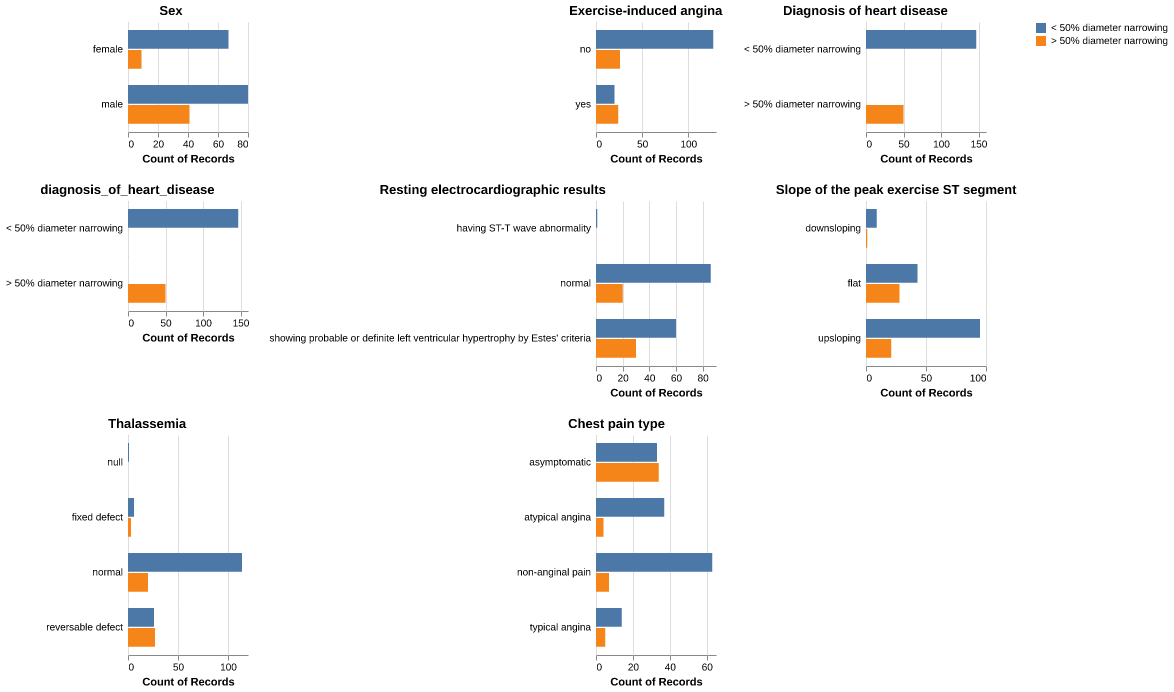
\includegraphics{../results/figures/categorical_distributions.png}

}

\caption{\label{fig-cat-dist}Distributions of Categorical Features}

\end{figure}%

\begin{figure}

\centering{

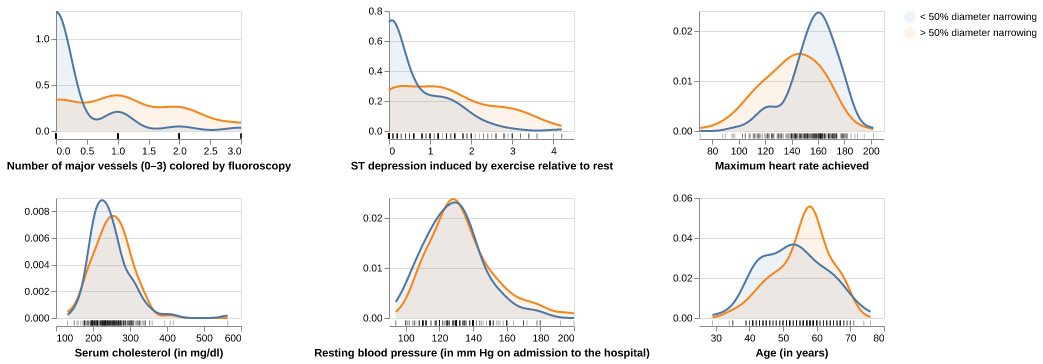
\includegraphics{../results/figures/numeric_distributions.png}

}

\caption{\label{fig-num-dist}Distributions of Numeric Features}

\end{figure}%

\begin{figure}

\centering{

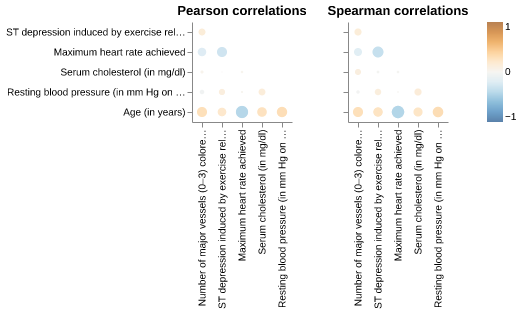
\includegraphics{../results/figures/correlation_matrix.png}

}

\caption{\label{fig-cor-mat}Correlation Matrix}

\end{figure}%

\subsubsection{4.2 ML-Analysis}\label{ml-analysis}

The following section outlines the procedure taken in creating our model
and testing it on our data set. As this is a classification problem
(predict whether the patient has the disease or not), the chosen models
for testing in this analyis are a Logistic Regression model and a Suport
Vector Classifier. These two models were selected as they have been
shown to historically perform well on real world data sets.

Since this data set is somewhat unbalanced (\textasciitilde80/20 split
on non-disease vs disease), the primary scoring metric to evaluate these
models will be F1 score, though model accuracy is still taken into
consideration. Due to the nature of the analysis, special attention is
taken to minimize false negatives as they represent the most damaging
type of error (predicting that a patient is free of the disease when he
does in fact have it). To this effect, we look to maximize Recall.

The framework upon which this analysis is based has been adapted from
DSCI573 Lab1.

\paragraph{4.2.1. Data Preprocessing}\label{data-preprocessing}

Features are sorted by type, and a column transformer object is created.
on categorical columns, simple imputing is applied filling missing
values with the most frequently occuring value. One hot encoding is then
performed.

For numerical feature, standard scaling is applied to keep all features
within the same range

\includegraphics{.pdf} - table of data head

\paragraph{4.2.2. model creation}\label{model-creation}

Basic models (default hyperparameter values) are now generated. A dummy
model is first created to use as a baseline to use for comparison. Then,
a logistic regressor and support vector classifier model is created.
5-fold cross validation (CV) is performed on each model and scores are
returned.

As discussed above, F1 score is to be the primary metric to evaluate
model performance, with precision as a secondary metric. this is
reflected in the scoring metrics used in CV

Finally, a Confusion matrix is generated for each model to give an idea
of false positive vs false negative rate.

\paragraph{4.2.3. Balanced model testing}\label{balanced-model-testing}

Step 4.2.2 is repeated, this time creating balanced logistic regressor
and SVC models, with all other hyperparameters held the same. Confusion
matrices are once again generated. The goal of this step is to gain an
understanding of how much accuracy is sacrificed at the benefit of
improving F1 score.

\paragraph{4.2.4. Model Evaluation and
Selection}\label{model-evaluation-and-selection}

With baseline models created, they are evaluated according to the
criteria set above. CV scores of each model are presented below. First,
standard deviation is shown verify there are no abnormally performing
models. Scores are then presented in the table below

Comparing the metrics across models, Balanced logistic regression yields
the highest recall and with second to the highest f1\_score. For this
report, we choose to proceed with
\texttt{LogisticRegression(class\_weight="balanced")} and optimize the
f1 score metric along with optimizing recall as we want to minimize
False Negatives, which is more damaging in medical diagnosis than False
Positives.

\begin{longtable}[]{@{}
  >{\raggedright\arraybackslash}p{(\columnwidth - 10\tabcolsep) * \real{0.2500}}
  >{\raggedleft\arraybackslash}p{(\columnwidth - 10\tabcolsep) * \real{0.1324}}
  >{\raggedleft\arraybackslash}p{(\columnwidth - 10\tabcolsep) * \real{0.1471}}
  >{\raggedleft\arraybackslash}p{(\columnwidth - 10\tabcolsep) * \real{0.1029}}
  >{\raggedleft\arraybackslash}p{(\columnwidth - 10\tabcolsep) * \real{0.2059}}
  >{\raggedleft\arraybackslash}p{(\columnwidth - 10\tabcolsep) * \real{0.1618}}@{}}

\caption{\label{tbl-model-cv-comps}Comparison of cross-validation scores
across model options.}

\tabularnewline

\toprule\noalign{}
\begin{minipage}[b]{\linewidth}\raggedright
index
\end{minipage} & \begin{minipage}[b]{\linewidth}\raggedleft
dummy
\end{minipage} & \begin{minipage}[b]{\linewidth}\raggedleft
logreg
\end{minipage} & \begin{minipage}[b]{\linewidth}\raggedleft
svc
\end{minipage} & \begin{minipage}[b]{\linewidth}\raggedleft
logreg\_bal
\end{minipage} & \begin{minipage}[b]{\linewidth}\raggedleft
svc\_bal
\end{minipage} \\
\midrule\noalign{}
\endhead
\bottomrule\noalign{}
\endlastfoot
fit\_time & 0.001 & 0.01 & 0.012 & 0.007 & 0.006 \\
score\_time & 0.003 & 0.006 & 0.008 & 0.004 & 0.005 \\
test\_accuracy & 0.746 & 0.797 & 0.818 & 0.731 & 0.747 \\
train\_accuracy & 0.746 & 0.85 & 0.896 & 0.822 & 0.916 \\
test\_precision & 0 & 0.638 & 0.824 & 0.477 & 0.524 \\
train\_precision & 0 & 0.789 & 0.969 & 0.609 & 0.779 \\
test\_recall & 0 & 0.44 & 0.38 & 0.68 & 0.62 \\
train\_recall & 0 & 0.56 & 0.61 & 0.84 & 0.94 \\
test\_f1 & 0 & 0.517 & 0.512 & 0.555 & 0.563 \\
train\_f1 & 0 & 0.655 & 0.747 & 0.706 & 0.851 \\

\end{longtable}

\subsubsection{4.2.5. Hyperparameter
optimization}\label{hyperparameter-optimization}

Proceeding with a balanced logistic regressor model, we now perform
hyperparameter optimization. Logistic regressors has only one
hyperparameter C, which is sampled from a loguniform distribution.
optimization is based on F1 score

The hyperparameter optimization made a difference
\textbf{(`mean\_test\_score' (0.58) {[}inline code{]} compared to
`mean\_test\_score of cross' (0.54) {[}inline code{]} of previous mean
validation score)}. However, the cross-validation scores among the top
three models are approximately equivalent. This suggests that the
model's performance is relatively stable across the parameter space,
indicating that further tuning may not yield substantial improvements.

\paragraph{4.2.6. Final model Scoring and
Evaluation}\label{final-model-scoring-and-evaluation}

With hyperparameters selected the best model is fitted on the training
set, then scored on both data sets. F1 score, Recall score and Accuracy
are all computed across both data sets.

\begin{figure}

\centering{

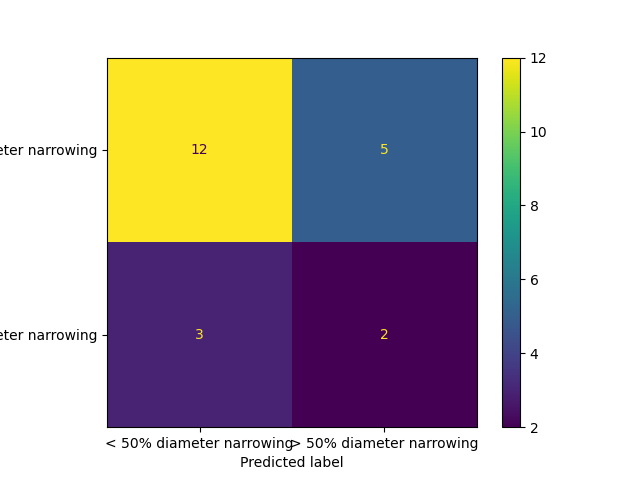
\includegraphics{../results/figures/confusion_matrix.png}

}

\caption{\label{fig-conf-mat}Confusion Matrix on Test Data}

\end{figure}%

\begin{longtable}[]{@{}lrr@{}}

\caption{\label{tbl-model-results}Best model metrics.}

\tabularnewline

\toprule\noalign{}
Metric & Train & Test \\
\midrule\noalign{}
\endhead
\bottomrule\noalign{}
\endlastfoot
F1 Score & 0.627 & 0.333 \\
Recall & 0.74 & 0.4 \\
Accuracy & 0.777 & 0.636 \\

\end{longtable}

\subsection{5. RESULTS \& DISCUSSION}\label{results-discussion}

The model created is promising. Applying it on our data set gave
approximately 63.6 percent accuracy. This value is close to our baseline
dummy accuracy, however with hyper parameter tuning the model achieved a
higher F1 score compared to original model (0.627 on train F1 score
compared to 0.555 F1 score for base model cv score). The final F1 score
on test data is found to be 0.333. Most importantly for our application,
the final model performed moderately well at minimizing false
negatives.\\
On our testing data set, the model performed moderately well, returning
a recall value of 0.4. The discrepancy between training and testing
score may be due to the fact that the test data set was quite small (22
examples). To get more rigorous performance testing and confidence in
our result, it would be recommended to seek further data.

\subsection{6. CONCLUSION}\label{conclusion}

The model created showed some promise, being able to correctly classify
presence of angiographic coronary disease with a decent level of
accuracy (63.6 percent). As well, the model performed moderately well on
F1 score and was able to minimize the number of false negatives
classified (recall of 0.4).

There are some limitations to this report that should be noted both at
the analysis level and application level.

On the analysis side, only 2 models were tested. While their performance
was encouraging, a more rigorous approach would test a variety of
classifiers before proceeding with logistic regression.

As well, further hyperparameter optimization could be conducted. While a
wide range of C-values were tested, Only 50 possible values were tested
from this range. An improvement to this would be to randomly sample from
a log-uniform distribution to obtain our best C value.

Lastly and perhaps most importantly, there is a large discrepancy
between our test data set relative to the training data. The most
reasonable explanation for this would be an test set too small to be
representative.

On the application side, we should note that this model was tested
specifically for one type of heart disease. The scope of the data used
in training should be taken into account before proceeding with
prediction on new data. As well this model requires a significant amount
of medical information about a patient in order to create a prediction.
Most of the information used to create the features to train the model
is obtained through angiography, a process which itself ends in a
diagnosis of the disease. So it is worth noting that even a high
performing model will not be immediately applicable, though it gives
confidence on the process.

Overall, we recommend further pursuing optimization of this model. Due
to the high discrepancy between training and testing scores, we would
strongly recommend performing further testing on the model on new,
larger data sets before proceeding with it.

\subsection*{7. REFERENCES}\label{references}
\addcontentsline{toc}{subsection}{7. REFERENCES}

\phantomsection\label{refs}
\begin{CSLReferences}{1}{0}
\bibitem[\citeproctext]{ref-thalassemia}
Athanasios Aessopos, Dimitrios Farmakis, Maria Kati. 2007. {``Heart
Disease in Thalassemia Intermedia: A Review of the Underlying
Pathophysiology.''} \url{https://haematologica.org/article/view/4438}.

\bibitem[\citeproctext]{ref-heart_disease_45}
Janosi, Steinbrunn, Andras, and Robert Detrano. 1989. {``{Heart
Disease}.''} UCI Machine Learning Repository.

\bibitem[\citeproctext]{ref-asymptomatic_coronary_disease}
Master, Arthur M. 1969. {``The Extent of Completely Asymptomatic
Coronary Artery Disease.''}
\url{https://doi.org/10.1016/0002-9149(69)90064-2}.

\bibitem[\citeproctext]{ref-OFlaherty2008}
O'Flaherty, M, E Ford, Steven Allender, P Scarborough, and S Capewell.
2008. {``{Coronary heart disease trends in England and Wales from 1984
to 2004 : concealed levelling of mortality rates among young adults},''}
January.
\url{https://dro.deakin.edu.au/articles/journal_contribution/Coronary_heart_disease_trends_in_England_and_Wales_from_1984_to_2004_concealed_levelling_of_mortality_rates_among_young_adults/21047827}.

\end{CSLReferences}




\end{document}
